\documentclass[letterpaper, 12pt, landscape]{ProgressBook}

\title{C\&O Progress}

\begin{document}

\fancyhead{} % clear all header fields
\chead{\makebox[\textwidth][c]{Daniel V Alhadeff and Alexandra Frackelton -- Spring 2019}}
\cfoot{\makebox[\textwidth][c]{\thepage}}

\begin{titlingpage}

  \let\footnotesize\small
  \let\footnoterule\relax
  \let \footnote \thanks
  \null\vfil
  \begin{center}
	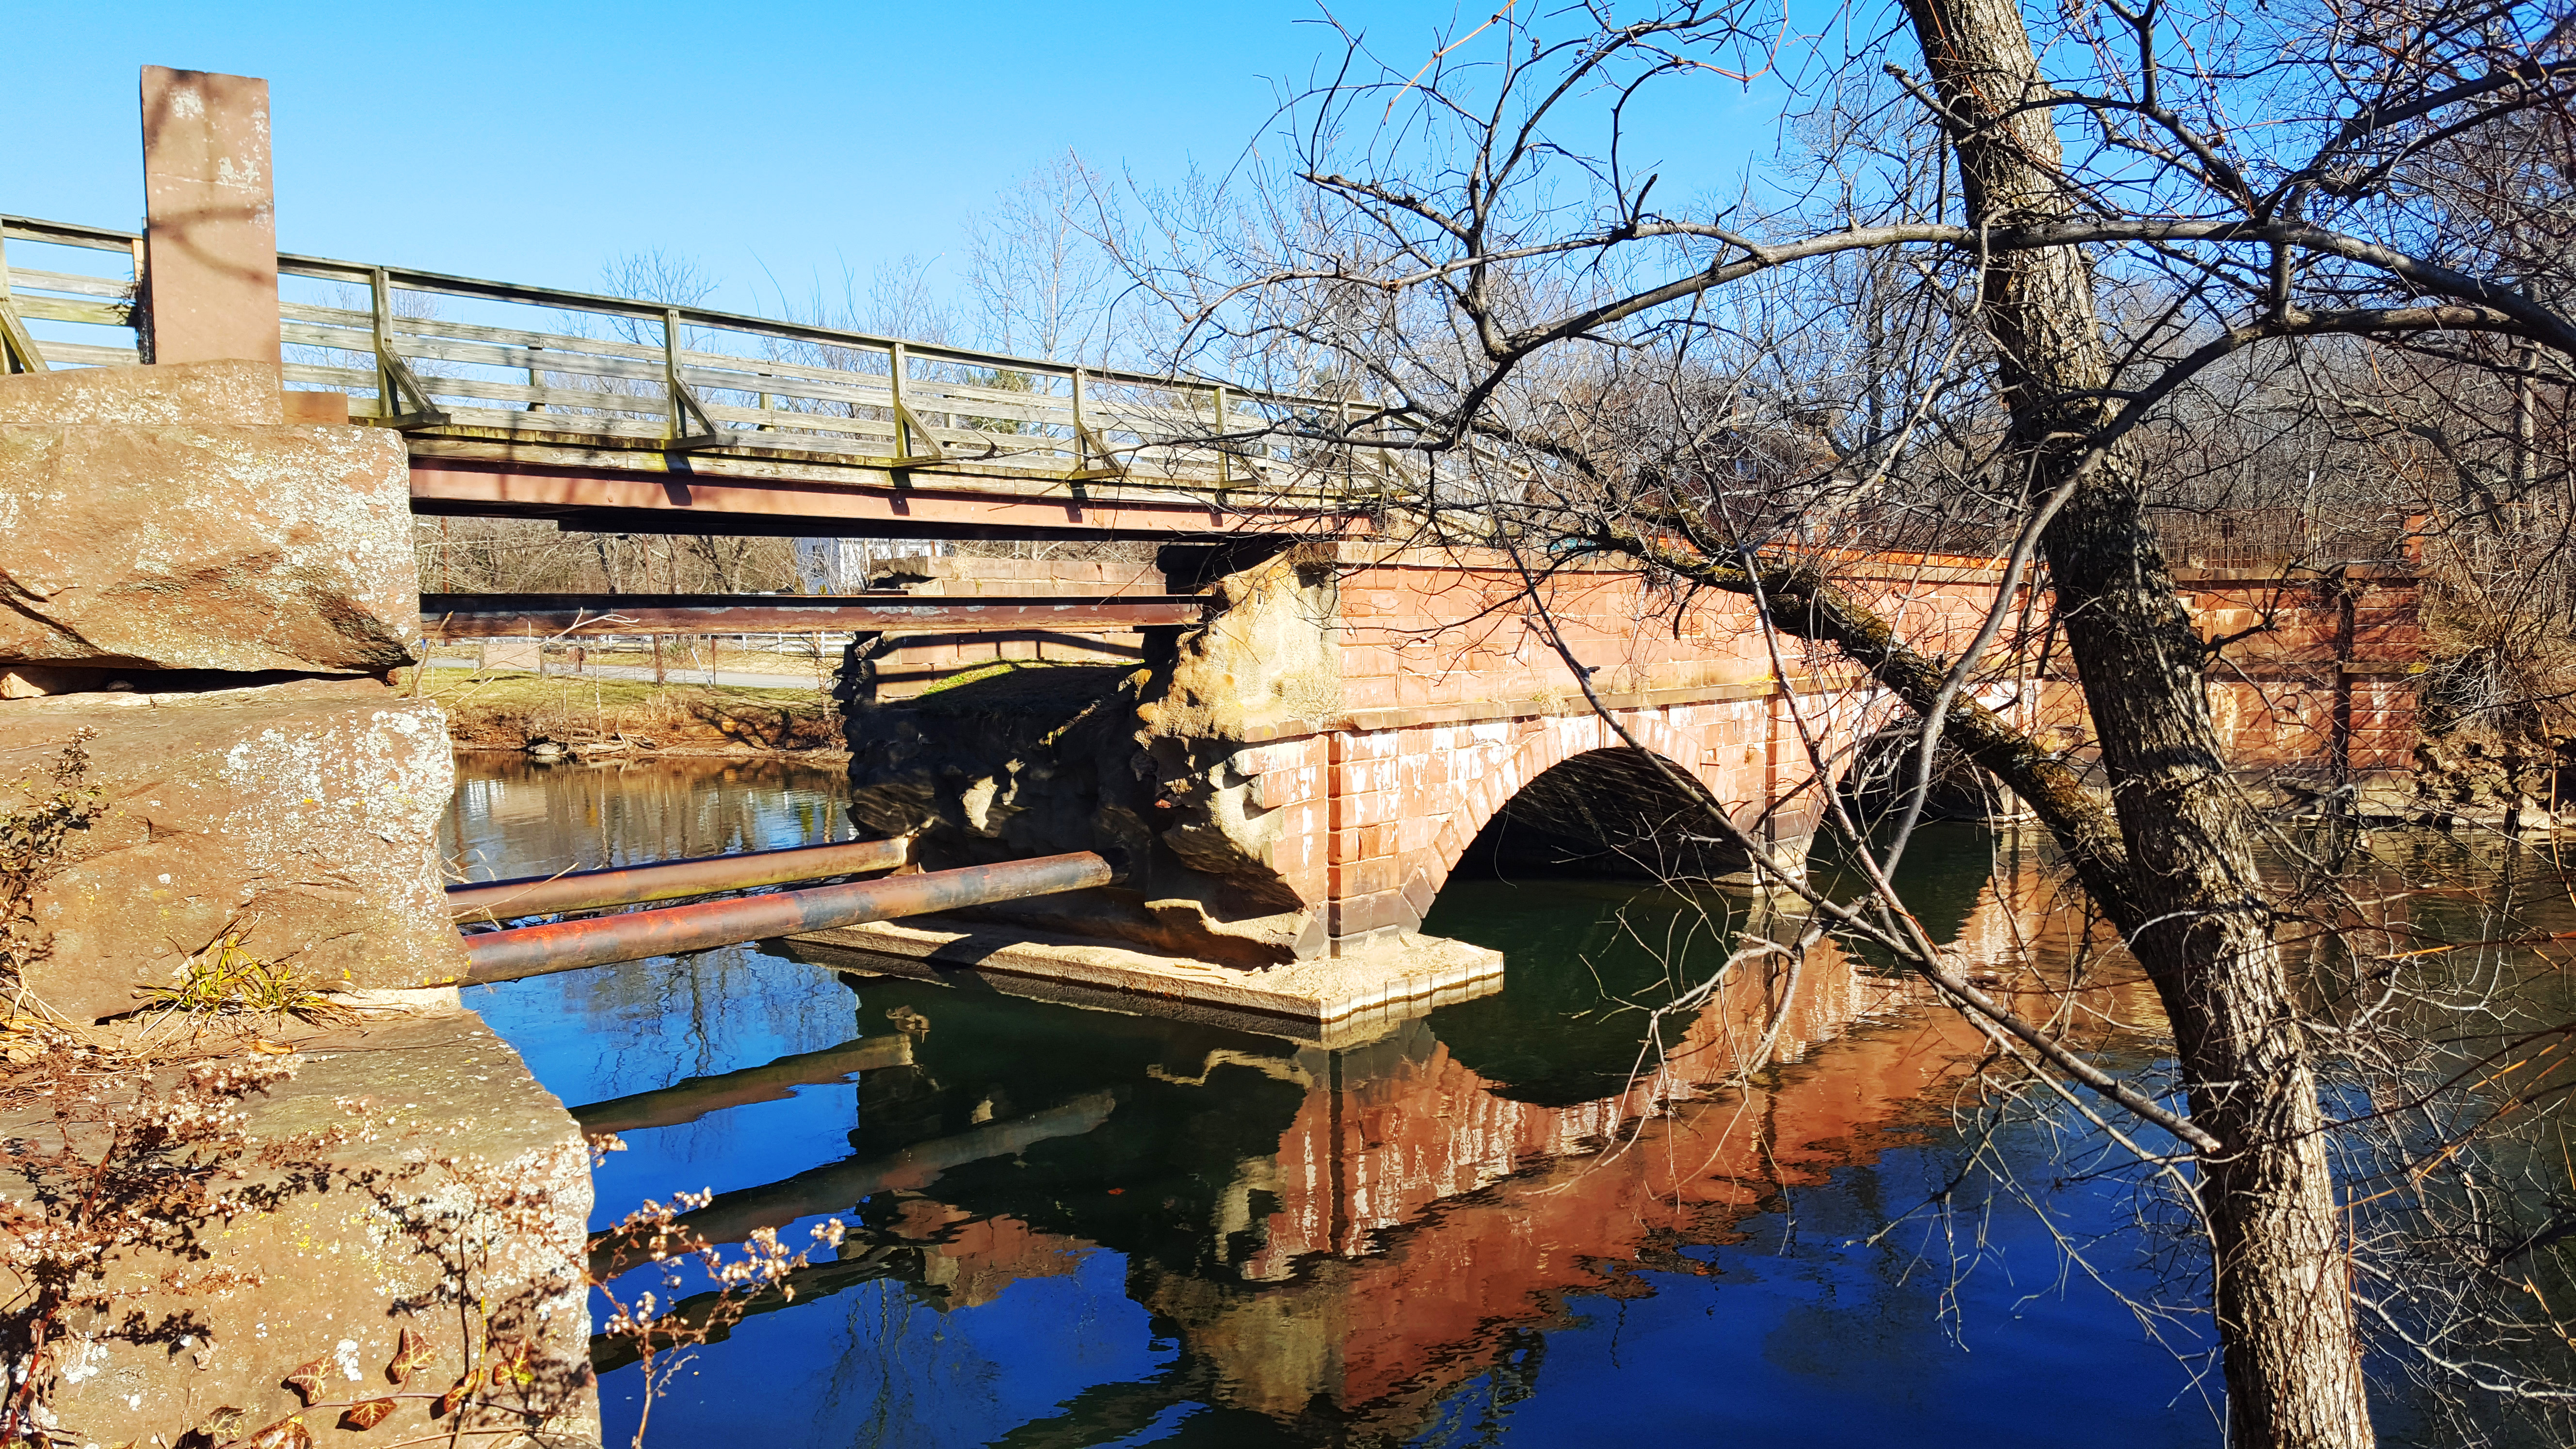
\includegraphics[max size={.85\textwidth}{.85\textheight}]{RileyAqueduct.jpg}
	\vskip 2em
	{\LARGE C\&O Drawing for Zan Frackelton}
  \end{center}
  \setcounter{footnote}{0}

  \end{titlingpage}

\section*{Summary}

On Sunday, February 25, 2018, I officially
proposed marriage to Zan. We have known each other since graduate school, and –
after digging through our Facebook chat history – have corresponded since about
2012. She and I reconnected in early 2016 and dated long-distance through a
weekly Facebook video chat call, until she moved to Maryland from Seattle in
2017.

When I proposed to her, I mentioned – off-handedly – that there
was an `invitation' still in the ‘mail’. This drawing is that official,
``engraved'' invitation to join me on a collective journey. The text, written in
Solitreo script, is the first line of a Ladino wedding folksong:
``\textit{Scalerica de oro i de marfil, para que suvia la novia a dar kiddushin}''
``A little ladder of gold and ivory that the bride will climb to say the wedding blessings''.
This invitation to her expresses my past (the Mandraki/Rhodes
windmill), our present (in Maryland, represented by the Seneca Creek Aqueduct
and Riley’s lockhouse on the Chesapeake \& Ohio Canal Towpath), with a
‘doorway’ into our future journey.

Physically, the drawing is on a 30''x22'' sheet of Arches
140\# hot-press watercolor paper, my favorite paper throughout architecture
school. I used a variety of sketching pencils, all from the Faber-Castell 9000 series
(4B, HB, H, 2H, and 4H!); the ``Raw Umber'' Faber Castell Polychromos colored
pencil was used for the ladder; a brush-pen was used for the text.

\section*{History}

I wanted to produce some artwork in honor of the two of us - it's
been way too long since I've done an art-drawing of any significance - to
celebrate our engagement. I was already doing very preliminary drafts of this
in my sketchbook during our trip to Iowa (with the theme of medieval fortifications,
the above-mentioned folksong, and the iconic Mandraki windmills) and intended
to complete it by the time I proposed. Things accelerated a bit in the final
weeks of December, with `field visits'/runs to refresh my memories of the
aqueduct, research on HABS (Historic American Building Survey), and several
drafts in Revit and on trace paper.

This same time in December and January, Zan and I had some very
preliminary ``visioning'' discussions about ketubot. What it sort of
boiled down to - for our purposes here - was that either a sofer or
calligrapher would have to be responsible for writing the text. Since I
wouldn’t expect them to use Arches \#140 hot-press watercolor paper, this vision
would not necessarily be as ``compatible'' with my usual style of
graphite art.

I finally got organized to draft and render right around
Hanukkah/Christmas, and ensured I had at least the start of the supplies I
needed. In fact, I’ve been sneaking visits to Plaza Arts with the sheets of
Arches and a whole store’s worth of graphite drawing pencils home these past
months. I have kept the drawing and supplies at the office, lest she visit my
apartment and see my drafting board and accessories setup, etc.
I have tried to keep my phone and email and messaging clean of
progress photos. At first, I kept saying that ``work was picking up again''.
The work did get hectic starting in March, as finishing this drawing grew more
urgent.

\section*{Riley’s Lock and Lockhouse, Seneca Creek Aqueduct, canal boat}

The subject of the drawing is primarily Riley's lock and Seneca
Creek aqueduct on the Chesapeakea and Ohio Canal. I've been a fan of the
C\&O towpath trail since I moved here, and have spent a few lovely
afternoons with Zan, running, walking, and biking with her. We have also
enjoyed the canal boat ride offered at Great Falls.
This aqueduct is not watered - and is basically in `ruin' - I've
drawn it whole, with a boat traveling downstream towards the lock. Part of the
aqueduct is ``cut-away'' in section to show the boat and the inside of
the lock gate. Detailed drawings of the lock, aqueduct, and lockhouse are
available from the Library of Congress through the Historic American Building
Survey. The canal boat referenced is actually a passenger boat, but the designs
for all C\&O boats appeared fairly consistent from a brief survey on Google.
The lockhouse was rendered based on photos taken on-site.
The Park Service/Canal Trust is restoring the upstream
Conococheague Aqueduct and plans to water it for tours. The area around Seneca
Creek features red sandstone (used when building the Smithsonian Castle, e.g.)
and I had investigated using a sepia/umber tone for the aqueduct stone to
celebrate this. After several small-scale tests, however, the plan became to
keep the stone - and majority of the drawing - black and white.

\subsection*{Windmill}

The windmill depicted references the type of windmill built on the
Island of Rhodes. A measured survey found online was used to establish
dimensions and clarify materials.

\subsection*{Ladder}

The ladder, rendered in raw umber colored pencil, leads from the
bottom of the lock to the lockhouse. Several of these ladders – built into the
upstream lock gates – appear at various locations throughout the (lower) canal.
Here, it is the ``\textit{scalerica}'' -- ladder -- referred to in the song. Silhouettes of the two of
us appear in the doorway of the lockhouse.

\subsection*{Text}

The text from ``Scalerica'' is written in the solitreo script used
by Ladino-speaking Jews in Spain, Turkey, Rhodes, and other locations. I
decided to learn it - an alternative to the ‘usual’ block lettering, and the
more modern European Hebrew handwritten script, especially given the subject.
Professors Devin Naar and David Bunis based at the University of Washington
provided guidance and resources in both spelling (sort of re-reverse
transliteration) and writing.

\section*{Conclusion}

This is a drawing I hope will hang next to our Ketubah. I almost
``lost my mind'' several times when we've discussed vision and style for the
Ketubah itself in relation to other art we own/like - and when she said I ought to do a drawing for the invitations, I wanted to scream! I plan to present this to
her, framed on the 27th, with her father, my mom and aunts in attendance.

\eject

\regPage{01.jpg}
{Original concept sketch imagining Riley's lockhouse as a medieval Rhodesli fortress. It was unclear at this point how exactly to draw the aqueduct and the ladder appears very large and out of scale.}
{01-01-2018-12h04.jpg}{01-01-2018 - 12h04}
{01-02-2018-11h56.jpg}{01-02-2018 - 11h56}
{01-03-2018-21h39.jpg}{01-03-2018 - 21h39}
{Happy New Year! The rendering begins in earnest \ldots}

\regPage{03.jpg}{After finding the Historic American Building Survey (HABS) documentation and several field visits, sketch is refined (via Revit) to show an actual scale (3/8'' : 1'-0'').}
{01-05-2018-15h32.jpg}{01-05-2018 - 15h32}
{01-07-2018-14h31.jpg}{01-07-2018 - 14h31}
{01-08-2018-18h52.jpg}{01-08-2018 - 18h52}

\regPage{05.jpg}{Things start coming together with decisions about how to both cut through and expose the inside and outside of the aqueduct. I made some key preliminary decisions about pencil hardness/`tone color' and used the section cut to start showing a canal boat. There are still three windmills, but they are now on the other side of the drawing, disengaged fully from the lockhouse.}
{01-10-2018-17h39.jpg}{01-10-2018 - 17h39}
{01-12-2018-16h31.jpg}{01-12-2018 - 16h31}
{01-14-2018-11h37.jpg}{01-14-2018 - 11h37}
{Zan went to Chicago to help Gillian shop for a wedding dress. Daniel went to Atlanta to buy the ring for Zan.}

\regPage{DanZanBrunch-2018.jpg}{Zan took Daniel out for brunch for his 33\textsuperscript{rd} birthday!}
{01-24-2018-18h34.jpg}{01-24-2018 - 18h34}
{01-28-2018-09h08.jpg}{01-28-2018 - 09h08}
{01-29-2018-18h30.jpg}{01-29-2018 - 18h30}

\regPage{09.jpg}{Part of drawing is constantly looking back at what's already on the page and judging how to move it forward. While I never did full-scale tests (not even thumbnails) of the entire image, I did frequently mock-up areas of the drawing to see how things would work.
For example, I had entertained the idea of using a lot more color in the drawing to emphasize the reddish-toned Seneca stone. I didn't want to use
a literal red, so I kept thinking of some color near `sepia-toned'. At the end of the project, no color was used -- except for the ladder, but it's nice to have the idea that color could work on a different drawing.}
{01-31-2018-17h31.jpg}{01-31-2018 - 17h31}
{02-04-2018-20h51.jpg}{02-04-2018 - 20h51}
{02-08-2018-20h19.jpg}{02-08-2018 - 20h19}
{David Franco unexpectedly early emailed Daniel that the `ring was ready', and would be arriving by the first Wednesday in February.}

\regPage{06.jpg}{The first steps after returning from Iowa \ldots}
{02-11-2018-21h21.jpg}{02-11-2018 - 21h21}
{02-13-2018-19h07.jpg}{02-13-2018 - 19h07}
{02-15-2018-23h02.jpg}{02-15-2018 - 23h02}

\regPage{06.jpg}{The first steps after returning from Iowa \ldots}
{02-18-2018-10h12.jpg}{02-18-2018 - 10h12}
{02-18-2018-22h04.jpg}{02-18-2018 - 22h04}
{02-19-2018-21h54.jpg}{02-19-2018 - 21h54}

\regPage{06.jpg}{The first steps after returning from Iowa \ldots}
{02-20-2018-22h10.jpg}{02-20-2018 - 22h10}
{02-22-2018-22h23.jpg}{02-22-2018 - 22h23}
{02-27-2018-06h50.jpg}{02-27-2018 - 06h50}
{Daniel officially proposed to Zan February 25, 2018 on the Maryland Heights overlook near Harper's Ferry, WV }

\regPage{06.jpg}{The first steps after returning from Iowa \ldots}
{02-28-2018-08h41.jpg}{02-28-2018 - 08h41}
{03-01-2018-22h38.jpg}{03-01-2018 - 22h38}
{03-02-2018-07h33.jpg}{03-02-2018 - 07h33}

\regPage{06.jpg}{The first steps after returning from Iowa \ldots}
{03-04-2018-23h12.jpg}{03-04-2018 - 23h12}
{03-05-2018-07h12.jpg}{03-05-2018 - 07h12}
{03-06-2018-06h24.jpg}{03-06-2018 - 06h24}

\regPage{06.jpg}{The first steps after returning from Iowa \ldots}
{03-07-2018-00h36.jpg}{03-07-2018 - 00h36}
{03-07-2018-08h09.jpg}{03-07-2018 - 08h09}
{03-07-2018-21h25.jpg}{03-07-2018 - 21h25}

\end{document}